
\begin{elevator}[Planarity]
A planar graph is a graph that can be drawn in the plane without edges crossings. We look at relations between the number of faces, edges and vertices of a graph. 
We also associate to every graph a dual graph. 
We touch on how the faces relate to the cycle space construction from before, and show that certain graphs are not planar. 
\label{sec:planar:planar}
\end{elevator}

While a graph is an abstract object, in practice we work with drawings of graphs for our intuition. A planar graph is a graph we can draw without the edges crossing. 
This means that all of the data of the graph can be easily read off of the picture.
We probably won't ever use the actual definition of a planar graph, but it's good at least to write it down once:
\begin{definition}
 A \emph{planar representation} of a graph $G$ is a set of vertices $V\subset \R^2$ and a set of continuous arcs $\{f_e: I\to \R^2\}_{e\in E}$ indexed by $E$ such that
 \begin{itemize}
  \item 
    If $f_{e}(t)=f_{e'}(t')$ and $t, t'\neq 0,1$,  then $e'=e$ and $t=t'$. 
    This means that the paths corresponding to edges do not cross over the interiors.  
  \item 
    If $uv$ is an edge, then $f_{uv}(0)=u$ and $f_{uv}(1)=v$. 
    This means that the paths corresponding to each pair of vertices have endpoints on the appropriate vertices.
 \end{itemize}
\end{definition}
We say that a graph is \emph{planar} if it admits a planar representation.
Note that it is possible for a graph to have topologically non-isomorphic planar representations. 

\begin{examplefigureenv}[Same graph, different drawings]{191figures/embgraph_treerepresentations.tikz}	Even a graph as simple as a tree can admit different planar representations. The trees on the right are the same as graphs, but there is no way to distort the first diagram into the second without creating a crossing at some point. To capture the planar information of a graph combinatorially, one can use the data of a rotation system.
\end{examplefigureenv}
A planar representation of a graph gives us a new piece of data: the \emph{faces} of a graph. 
\begin{definition} A \emph{Face} of a planar representation of $G$ is a connected component of $\R^2\setminus G$.  The set of such components is denoted $F(G)$. 
\end{definition}
\nomenclature{$F(G)$}{The faces of $G$.}
 Notice that this definition gives us a large ``outer face'' to the graph. To each face, we get a \emph{closed walk} which makes up the boundary of the face. Even though a closed walk is not a cycle, it is an element of the cycle space. 
\begin{definition} Let $G$ be a planar graph with a fixed embedding, and let $F=\{f_1, \ldots, f_k\}$ be the set of faces. Let $\mathcal F$ be the $\Z_2$ vector space generated on the set $F$. Let $\partial_F: \mathcal F\to \mathcal E$ be the map which sends each face to the subset of edges in it's boundary (counted with multiplicity.) 
 \end{definition}
This is a construction very similar to those that we've employed for our algebraic analysis of graphs, just we've included faces into it. 
\begin{claim}
Consider the following sequence of vector spaces and functions:
\[ \begin{tikzcd}
\mathcal F \arrow{r}{\partial_F} & \mathcal E \arrow{r}{\partial_E} & \mathcal V
\end{tikzcd}\]
This is a \emph{chain complex}, in that $\partial_E\circ \partial_F =0$ \label{def:planarcomplex}
\label{claim:dsquarezerograph}
\end{claim}
\begin{proof}
In order to show that $\partial_E\circ \partial_F=0$, it suffices to check on a basis of $\mathcal F$. Let $f\in \mathcal F$ be a face. Then $\partial_F(f)$ is a union of cycles. By \ref{claim:cyclespaceisker}, this lies in the kernel of $\partial_E$. 
\end{proof}
We will develop the algebraic theory of chain complexes throughout the course-- for more details, see Appendix \ref{append:chaincomplexes}. 
We'll bring this complex back throughout this section.  Let's look at some basic facts about planar graphs.

A useful geometric construction for planar graphs is the \emph{dual graph} construction. Given a graph $G$ with a planar embeddings, we can construct a multigraph which is dual to it. 
\begin{definition}[Multigraph]
 A multigraph on $n$ vertices is a symmetric $n\times n$ matrix with entries in $\N$. 
\end{definition}
The coefficient in the $i,j$ spot of the matrix denotes the number of edges that lie between the $i $ and $j$ vertex. 

\begin{examplefigureenv}[Multigraph]{191figures/embgraph_multigraph.tikz}
  For example, here is the multigraph given by the matrix 
\[\begin{pmatrix}
0&2&0&0\\
2&0&1&3\\
0&1&2&1\\
0&3&1&0 \end{pmatrix}\]
\end{examplefigureenv}
Let $G$ be a planar multigraph. From here we can construct a new planar multigraph, called the \emph{dual} of $G$, interchanging the roles of vertices and edges. 
\begin{definition}
Let $G$ be a planar multigraph. Let $G^*$ be the graph where 
\[V(G^*)=F(G), E(G^*)=E(G), F(G^*)=V(G)\]
We have an edge between two vertices between $f_i$ and $f_j$, for each common edge in the boundary of the faces $f_i$ and $f_j$.
\label{def:dualgraph}
\end{definition}
\begin{examplefigureenv}[A graph and its planar dual]{191figures/embgraph_planarduals.tikz}
  An example of a graph $G$ in black and its corresponding dual multigraph $G^*$ in red. Notice that the degree of each vertex counts the number of edges in the boundary walk of the graph in the dual, and vice versa. Also notice that the double dual, $(G^*)^*$, is $G$. 
\end{examplefigureenv}
\nomenclature{$G^*$}{The dual graph to $G$}
One can similarly define the boundary maps and face maps to the theory of multigraphs, either by taking the counts of edges $\mod 2$ or by using \label{proj:dualsandhomology} \emph{directed multigraphs.} 


\begin{projectdescription}{Duals and Homology}
  In both cases, we see that the theory of planar graphs comes with two equally good chain complexes. On one hand, we can look at $\mathcal F(G)\to \mathcal E(G)\to\mathcal V(G)$. On the other hand, we might have instead of chosen to study $\mathcal F(G^*)\to \mathcal E(G^* )\to \mathcal V(G^*)$.
\end{projectdescription}
 By identifying $\mathcal F(G^*)=\mathcal V(G)$, we get a different set of maps:
\[ \begin{tikzcd}
\mathcal F& \arrow{l}{d_E} \mathcal E& \arrow{l}{d_V}  \mathcal V
\end{tikzcd}\]
which is a kind of ``dual complex'' to our original theory. 
\begin{claim}
If $G$ is a simple graph, then every vertex of $G^*$ has degree at least 3.
\end{claim}
\begin{proof}
This is because each vertex of $G^*$ corresponds to a face in $G$, and the boundary of such faces are cycles of $G$. Since $G$ is simple, each cycle must have length at least 3. This means that each face borders at least 3 other faces, so the degree of each $f_i\in V(G^*)$ must be at least 3. 
\end{proof}
\begin{claim}[Basic Graph Properties]
 Let $G$ be a connected simple planar graph, and let $V, E, F$ be the set of vertices, edges and faces. 
 \begin{itemize}
  \item $2|E|\geq |V|$
  \item $2|E|\geq 3|F|$
 \end{itemize}
\end{claim}
\begin{proof}
 The first claim follows from our argument about average degree and edges in Claim \ref{claim:avgdegree}. Since $G$ is connected, the average degree of a vertex is at least 1. \\
 The second claim is actually the same as the first claim, just applied to the dual graph. As every vertex in $G^*$ has degree at least 3, we have that 
 \[2E(G)=2E(G^*)=(\text{ Average degree in $G^*$ )}|V(G^*)|\geq 3|V(G^*)|= 3|F(G)|.\] 

\end{proof}
The structure of a graph gives us an additional relation between the number of vertices, edges and faces. 
\begin{theorem}[Euler's Formula]
Let $G$ be a connected planar graph. Then
  \[|V|-|E|+|F|=2.\]
  \label{thm:eulersformula}
\end{theorem}
\begin{proof}
 This theorem is traditionally prove by induction on the number of edges. Of course, we cannot induct on the number of edges right away, because if we remove an edge from a graph it may not remain connected. However, with every connected graph $G$, there exists an edge so that $G\setminus e$ is connected, or $G$ is a tree (See Exercise \ref{exer:tree}.) Therefore, checking trees suffices as a base case.\\
 In the case of a tree, we know that the number of edges is 1 fewer than the number of vertices, and the number of faces is 1. This gives us 
 \[|V|-|E|+|F|=|V|-(|V|-1)+1=2.\]
 For the induction step, let $G$ be a planar connected graph, and let $e$ be an edge so that $G\setminus e$ is still connected. Since $G\setminus e$ is still connected, it is the case that $e$ belongs to 2 different faces. Therefore, $E(G\setminus e)=E(G)-1$, and $F(G\setminus e)=F(G)-1$. We conclude that 
 \begin{align*}
 |V(G)|-|E(G)|+|F(G)|= &|V(G\setminus e)|-(|E(G\setminus e)|+1)+(|F(G\setminus e)|+1)\\
 =&|V(G\setminus e)|-|E(G\setminus e)|+|F(G\setminus e)|\\
 =&2.
 \end{align*}
\end{proof}
A nice way to prove this is to use the algebraic graph techniques that we've been working on. See Exercise \ref{exer:eulercharacteristic} for details on how one would prove this. 
\begin{corollary}
Let $G$ be a simple planar graph. If $|V|\geq 3$, then $|E|\leq 3|V|-6$. 
\label{emb:cor:inequality}
\end{corollary}
\begin{proof}
 Take a planar simple graph $G$ with at least 3 vertices. Suppose that it is not the case that every face of $G$ is a triangle. Then you may add an edge to $G$ and keep it planar whenever $G$ has a face which is not a triangle. When all of the faces of $G$ are triangular, the graph is \emph{maximally planar}.

 Let $G'$ be a maximally planar graph containing $G$. In this situation we have the additional equality $2|E(G')|=3|F(G')|$. From Euler's formula, we have 
 \[|V(G')|-|E(G')|+2/3 |E(G')|=2\]
Since $G'$ has more edges than $G$, we can rearrange this equality to $|E|\leq 3|V|-6$. 
\end{proof}
These simple inequalities already place many restrictions on a planar embedding for many graphs. For instance, in \sref{emb:exm:platonic} we use this classify the face and vertex regular planar graphs, i.e. the Platonic solids. 

The inequality also provides a criterion that can show the non-existence of any graph embedding. Roughly speaking, if your graph as many edges compared to vertices, it is unlikely that \sref{emb:cor:inequality} will be satisfied. As complete graphs maximize the edge-to-vertex ratio, they are a natural first candidate to check. 

\begin{corollary}
 For every $n\geq 5$, the complete graph $K_n$ admits no planar embedding. 
\end{corollary}

\begin{proof}
 It suffices to show this for $n=5$, as an planar embedding of $K_n$ with $n>5$ induces a planar embedding of $K_5$.  For $K_5$, we have that $|E|=10$, and $|V|=5$. This fails to satisfy $|E|\leq 3|V|-6$. Therefore $K_5$ is nonplanar. 
\end{proof}
This gives us actually a general criterion we can check to see if a graph is non-planar, as if even $G$ contains $K_5$ as a topological minor, it cannot be planar. 


\begin{framedpage}{Example}{The Platonic Solids}{
 The only Platonic solids are the tetrahedron, cube, octahedron, dodecahedron or icosahedron. \label{emb:exm:platonic}
}
 Recall that a Platonic solid is one where all the vertices have the same degree and all of the faces have the same number of edges. We can take any polyhedron and convert it into a planar graph by stereographic projection. Therefore, to each platonic solid we should look at a graph which has vertices of degree $m$, and faces $n$ boundary edges. \\
 Since we know the degree and size of each edge, we can state the exact relations:
 \[2|E|= n|F|\]
 \[2|E|= m|V|\]
 Therefore, $|F|=m/n|V|.$ Applying this to Euler's formula tells us:
 \[|V|-m/2|V|+m/n|V|=2\]
 Now, we have some additional geometric bounds we may place  on $m$ and $n$. 
 \begin{itemize}
  \item We know that $n$ is at least 3 (all faces have at least 3 sides.)
  \item We get the bound \[m\left(\frac{1}{n}-\frac{1}{2}\right)> -1\] from the Euler characteristic formula. This means that $m$ cannot be greater than $5$.
  \item $m$ must be at least 3. The only valid values of $m$ are now 3, 4, 5. 
  \item By taking a dual polygon, we get similar restraints on $n$. 
 \end{itemize}
Tabulating our results we have:
\[
 \begin{tabular}{c|c|c|c|c|c}
   $m$ & $n$ & $|V|$ & $|E|$& $|F|$ & Shape\\ \hline
   3 & 3& 4& 6 & 4 & Tetrahedron \\
   3& 4& 8& 12& 6 & Cube\\
   3& 5& 20& 30 &12 & Dodecahedron\\
   4& 3& 6&12 & 8 & Octohedron \\
   5& 3& 12& 30 & 20 & Icosohedron\\   
 \end{tabular}
\]
There is a kind of duality that you might notice here on first inspection. First of, in the proof, it seems like the values of $m$ and $n$ are exchangeable. This is reflected in the platonic solids that we've found- they come in pairs where the roles of vertices and faces are reversed. These dual-polytopes pairs are given by dual-graphs. 


\end{framedpage}


\begin{projectdescription}{Polyhedra}
  Outside of the Platonic solids, there are many different types of polytopes that one can study and represent with graphs. For instance, a \emph{quasi-regular} polyhedra is allowed to have 2 different kinds of faces that alternate \label{proj:polytope} around each vertex, and their classification follows a similar argument as the one used above. The general theory of understanding convex polytopes branches substantially into algebraic topology. For instance, understanding the simplicial convex $d$-polytopes can be understood in just the number of facets it has in every dimension( \cite{stanley1980number}). 
\end{projectdescription}


\begin{elevator}[Graph Colorings]
We return to a historic problem: how many colors are needed to color a map. We first explore abstract colorings of maps, including coloring estimates, chromatic polynomials, and properties of 2-colorable graphs. We then later turn to coloring planar graphs, proving the 6 and 5 color theorem. 
\end{elevator}
\label{sec:planar:coloring}
We're going to take a slight detour from planar graphs to talk about graph colorings, which are a major tool in graph theory. Eventually, we'll bring this back to planar graphs when we discuss colorings of planar graphs. 
\begin{definition}[Colorings]
 Let $G$ be a graph. A \emph{$k$-coloring} of a graph $G$ is an assignment  $f: V\to \{1,2, \ldots ,k\}$ such that if $xy\in E$, $f(x)\neq f(y)$. The minimal $k$ such that a $k$ coloring of $G$ exists is called the \emph{chromatic number} of $G$ and is denoted $\gamma(G)$. 
\end{definition}

\nomenclature{$\gamma(G)$}{The chromatic number of $G$}
\begin{examplefigureenv}[Coloring a graph]{191figures/embgraph_4colors.tikz}
  The graph on the right, despite not containing a complete graph on 4 vertices, still requires a minimal of 4 colors to color. The proof is as follows: the colors of the top 5 vertices are fixed because it is constructed out of triangles. We are thus forced to paint the final leftmost vertex a fourth color. The removal of the dashed edge would lower the chromatic number to 3. 
\end{examplefigureenv}
Colorings, like connectivity, are both influenced by local properties of the graph and by global properties of the graph. For instance, a local result is:
\begin{claim}
 Let $\Delta(G)$ be the maximal degree of vertices in $G$. Then $G$ admits a $\Delta+1$ coloring. 
\end{claim}
A global result on coloring is:
\begin{claim}
 Let $G$ be a graph. Then 
 \[\gamma(G)\leq \frac{1}{2}+\sqrt{2|E|+\frac{1}{4}}\]
\end{claim}
\begin{proof}
\begin{paragraphfigureenv}{191figures/embgraph_nonOptimalColoring.tikz}
 Create a multigraph $K_G$ on $\gamma(G)$ vertices, where each vertex represents one color class from $G$, and you draw an edge between two vertices if the color classes have an edge between them. If this is an efficient coloring, then this multigraph must have edges between every two color classes; otherwise those classes could be labeled the same way (see Figure \ref{fig:nonoptimalcolor} for an example of these graphs.) Since this is a complete graph on $\gamma(k)$ vertices, $G$ must have at least $\frac{1}{2}k(k-1)$ edges. 
\end{paragraphfigureenv}
\end{proof}
In fact, we can improve our local result on coloring by 1, see \sref{emb:thm:brooks}. 

It turns out that neither global or local results allow us to pin down the colorability of a graph. Neither will information on the connectivity of a graph. For example:
\begin{itemize}
 \item Average degree does not give us a good pin on chromaticity. Take, for instance, a graph that has a $K_n$ subgraph but then a huge number of free-floating vertices. This is $n$ colorable, although the average degree is very small. 
 \item Connectivity does not give us a good pin on chromaticity. Take, for instance the complete bipartite graph on $n$ and $n$ vertices: this is a graph with vertices $v_1, \ldots v_n, w_1, \ldots w_n$ with edges $w_iv_j$ for every $i, j$. This graph is $n$ connected, but is 2-colorable. On the other hand, a tree is a 2 connected graph which is also 2 colorable. 
\end{itemize}
\begin{doubledpage}{theorem}{Brook's theorem \cite{brooks1941colouring}}{ 
  Let $G$ be a connected graph which is not an odd cycle or a complete graph. Then $\gamma(G)\leq \Delta(G)$. \label{emb:thm:brooks}}


The basic observation in this proof is that you can switch two colors in a graph coloring and still wind up with a valid graph coloring. 

 We induct on the number of vertices. The base case is to look at the trivial graph, and it follows trivially. 

  Now for the inductive step, assume that $G\setminus v$ satisfies the theorem by induction hypothesis. If $v$ has degree less than $\Delta(G)$, then we can color it greedily; therefore we should assume that $v$ is a vertex of degree $\Delta(G)$. We may also make the assumption that the neighbors of $v$ do not make a complete graph. 
  
  Given a coloring of $G\setminus v$, we get a $\Delta(G)$-coloring of $G$. We now have 2 cases:

 \textbf{Case 1:} Suppose that 2 of the neighbors of $v$ are colored with the same color. Then not all $\Delta(G)$-colors are used in $N(v)$, so we may color $v$ with the remaining color. 
 
 \textbf{Case 2:} We are now in the harder case, where $N(v)$ is uses every color. We therefore may index the points in the neighborhood of $v$ by the color set: with this labeling, $N(v)=\{v_1, \ldots, v_\Delta\}$. We want to show that we can simplify this coloring. For our construction,  $H_{i,j}$ be the subgraph of $G\setminus v$ which has been colored by $i$ and $j$. Here are some simple cases that we can rule out: 
 
\begin{paragraphfigureenv}{191figures/topgraph_colordegree1.tikz}
\textbf{Easy Case:}Suppose that for some $i, j$, $v_i$ and $v_j$ do not lie in the same connected component of $H_{i,j}$. Then let $C^i_{i,j}$ be the connected component of $H_{i,j}$ containing $v_i$. On this subgraph, switch the colors of $i$ and $j$. Now this produces a valid coloring on $G\setminus v$, and the vertex $v_i$ will now be colored $j$. Now we can color the vertex $v$ the color $i$.  
\end{paragraphfigureenv}


\begin{paragraphfigureenv}{191figures/topgraph_colordegree2.tikz}
\textbf{Easy Case:} Additionally, we may assume that the connected component containing $v_i$ and $v_j$ is a path. If it wasn't a path, then there is a vertex $w$ that has degree 3 in the path. Necessarily, one of $N(w)$ is not colored with $i$, $j$ or some other color $k$. Color $w$ with the color $k$ instead. With this updated coloring, we have that $H_{ij}$ separates the vertices $v_i$ and $v_j$, and we may apply the previous easy case. 
\end{paragraphfigureenv}


\begin{paragraphfigureenv}{191figures/topgraph_colordegree3.tikz}
  \textbf{Ease Case:} For any $i, j, k$, the paths we've constructed from $v_i$ to $v_j$ and from $v_j$ to $v_k$ may only intersect at $v_j$. Any other intersection point $w$ would have two neighbors colored $i$, and two neighbors colored $k$, and could therefore be colored some other 4th color
\end{paragraphfigureenv}


Since the neighbors of $v$ do not make a complete graph, we can assume without loss of generality that $v_1v_2$ is not an edge of $G$.  Let $P_{12}$ be the path from $v_1$ to $v_2$. 
Let $w$ be a point on that path closest to $v_1$ (this point will be colored $2$. ) \\
We now will generate a new coloring for $G$ by switching colors 1 and 3 in the path from $v_1$ to $v_3$. I'll label the changed color vertices with parenthesis. Take a look at Figure \ref{fig:brooks} for pictures.

\begin{figure}[h]
  \newcommand{\vertexradius}{2.5pt}
\newcommand{\vertexscale}{.5}
\newcommand{\bigvertexscale}{1}
\newcommand{\vertex}{\node[circle, fill=black, scale=\vertexscale] }
\newcommand{\highlighta}{red!20}
\newcommand{\highlightb}{blue!20}
\newcommand{\highlightc}{green!20}
\newcommand{\shadinga}{gray!20}
\newcommand{\smallvertex}{\node[circle, fill=black, scale=.2]}
\newcommand{\highlightlinewidth}{3pt}

\tikzset{every path/.style={line width=1 pt}}
\centering
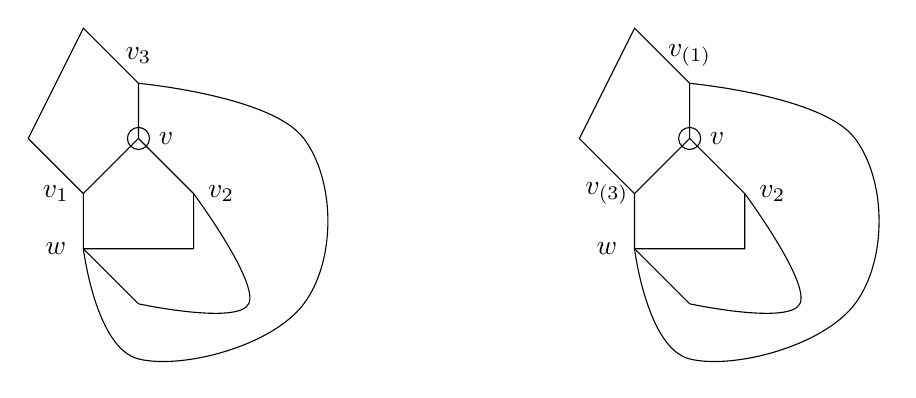
\begin{tikzpicture}[scale=.7]

\draw (5,0) circle[radius=.2];

\draw (5,0) -- (4,-1) -- (3,0) -- (4,2) -- (5,1) -- (5,0);
\draw (4,-1) -- (4,-2) -- (6,-2) -- (6,-1) -- (5,0);


\draw (-5,0) -- (-6,-1) -- (-7,0) -- (-6,2) -- (-5,1) -- (-5,0);
\draw (-6,-1) -- (-6,-2) -- (-4,-2) -- (-4,-1) -- (-5,0);
\draw (-6,-2) -- (-5,-3);
\draw  plot[smooth, tension=.7] coordinates {(-5,-3) (-3,-3) (-4,-1)};
\draw (4,-2) -- (5,-3);
\draw  plot[smooth, tension=.7] coordinates {(5,-3) (7,-3) (6,-1)};
\draw  plot[smooth, tension=.7] coordinates {(4,-2) (5,-4) (8,-3) (8,0) (5,1)};
\draw  plot[smooth, tension=.7] coordinates {(-6,-2) (-5,-4) (-2,-3) (-2,0) (-5,1)};
\node at (-6.5,-1) {$v_1$};
\node at (-6.5,-2) {$w$};
\node at (-5,1.5) {$v_3$};
\node at (-3.5,-1) {$v_2$};
\node at (-4.5,0) {$v$};
\node at (3.5,-1) {$v_{(3)}$};
\node at (3.5,-2) {$w$};
\node at (5.5,0) {$v$};
\node at (5,1.5) {$v_{(1)}$};
\node at (6.5,-1) {$v_2$};\vertexc at (4,2) {};
\vertexb at (4,-2) {};
\vertexa at (3,0) {};
\vertexa at (6,-2) {};
\vertexa at (5,1) {};
\vertexb at (6,-1) {};
\vertexc at (4,-1) {};
\vertexc at (5,-3) {};
\vertexc at (-5,-3) {};
\vertexa at (-6,2) {};
\vertexb at (-6,-2) {};
\vertexc at (-7,0) {};
\vertexa at (-4,-2) {};
\vertexc at (-5,1) {};
\vertexb at (-4,-1) {};
\vertexa at (-6,-1) {};
\draw (-5,0) circle[radius=.2];
\end{tikzpicture}
\caption{Recoloring path segment to simplify the coloring.}
\label{fig:brooks}
\end{figure}
With this new set-up $w$ is in the connected component from $v_1=v_{(3)}$ to $v_2$, and is still colored 2.\\
In this new coloring look at the $\{1, 2\}$ colored path between $v_2$ and $v_{(1)}$ The vertex $w$ must belong to this new path. Since $w\in N(v_{(3)})$, we must additionally also have that $w$ is in the $\{2, 3\}$ colored path between $v_{(3)}$ and $v_2$. \\
This means that $u$ belongs to 2 paths. This means that we are in the 3rd kind of easy case, and we can simplify our coloring. 
 


\end{doubledpage}
Indeed, even local structure does not give us a good pin on chromaticity. Take for instance this theorem of Erd\"os:
\begin{theorem}[\cite{erdos1960graph}] \label{proj:probmethod}
 There exists a graph $G$ which contains no cycles of size smaller than $d$, but has a chromatic number at least $k$, for every $d$ and $k$. 
\end{theorem}
\begin{projectdescription}{Probabilistic method}
In order to prove this, Erd\"os used a technique called the probabilistic method. This technique allows you prove the existence of certain combinatorial object by arguing that the probability of them existing in a randomly generated combinatorial object is non-zero. In this case, Erd\"os 
let $G_{n,p}$ be a graph on $n$ vertices with each edge appearing with probability $p$. He then shows there exists $(n, p)$ so that the probability that $G_{n,p}$ has a small cycle and is colorable by few colors is less than 1. 
Even though this method proves the existence of such a sparse-highly colored graph, it is in practice difficult to construct such a graph. 
\end{projectdescription}

For all of these difficulties, we expect that chromatic number of graph is a rather mysterious value to get a good pin on. However, we have a deletion-contraction tool which gives us an algorithem for computing the chromatic number of a graph.  
\subsection{Chromatic Polynomial}
Colorings of graphs follow some nice algebraic properties:

\begin{definition}[Chromatic Polynomial]
 Let $G$ be a graph. For $k\geq 0$, define $P_G(k)$ to be the number of $k$ colorings of $G$. 
\end{definition}
As the name suggest, the chromatic polynomial is a polynomial. 
\begin{theorem}
 $P_G(k)$ is a polynomial with integer coefficients of degree $|V_G|$. 
\end{theorem}
\begin{proof}
 We prove a stronger statement, that the chromatic polynomial satisfies the recursive relation:
 \[P_G(k)=P_G{G\setminus xy}(K)- P_{G/xy}(K)\]
 for any edge $xy$. This along, with the knowledge that if $H_n$ is the graph with $n$ vertices and no edges, then $P_{H_n}(k)=k^n$, will prove that $P_G(k)$ is a polynomial with integer coefficients. \\
 The proof of the statement is now quite easy-- note that colorings of $G$ are in bijection with colorings of $G\setminus xy$ where $x$ and $y$ do not have the same color. Further, colorings of $G\setminus xy$ where $x$ and $y$ do have the same color are in bijection with $G/xy$. This finishes the proof. 
\end{proof}
This may look similar to the method that we used for the Reliability polynomial, and indeed it is. There are several other graph properties which can be computed by ``deletion-contraction'' type relations. \\
The chromatic polynomial satisfies some very unusual properties:
\begin{theorem}[\cite{thomassen1997zero}]
 The zeros of the chromatic polynomials cannot occur in the interval $[-\infty, 32/27]\setminus \{0, 1\}$, and are dense everywhere else on the real line.
\end{theorem}
\begin{projectdescription}{Zeros of the Chromatic Polynomial}
  Interestingly, the roots of chromatic polynomials do not give us all of the algebraic numbers. For instance $\phi+1$ may never be the root of a chromatic polynomial (where $\phi$ is the golden ratio). However, the set of all roots of chromatic polynomials is dense in $C$. The properties of roots chromatic polynomials is still not completely understood.
  \end{projectdescription}

\subsection{Bipartite Graphs}
 However, colorings of graphs have some unexpected properties. Many properties of graphs are easier to compute. One particularly useful thing to know is if a graph is 2-colorable. In this case, we call the graph \emph{bipartite.}
\begin{claim}
 A graph $G$ is bipartite if and only if all of its cycles are even length. 
\end{claim}
\begin{proof}
 The right direction is easy. Take any cycle, and try to color it with two colors-- this is only possible if the cycle has an even number of verticals. \\
 For the other direction, take any vertex $v\in G$. Without loss of generality, let $G$ be connected. For any vertex $w$, take a path $P_w$ from $v$ to $w$. If $P_w$ has even length, color $w$ white, otherwise color $w$ black. As all cycles are of even length, the parity of the length of $P_w$ is independent of path chosen. 
\end{proof}

\begin{claim}
 The maximal number of edges in a bipartite graph with at most $n$ vertices if $\lfloor n/2 \rfloor \lceil n/2 \rceil$. 
\end{claim}

In bipartite graphs, we have another min-max result similar to the min-max result that we saw for connectivity. 
	\begin{theorem}[\cite{konig1916graphok}]
 Let $G$ be a bipartite graph. Let $U\subset V$ be a subset minimal with respect to the property that every vertex of $v$ has a neighbor in $U$.  Let $F\subset E$ be a subset of edges maximal with respect to the property that all edges of $f$ are disjoint. Then $|U|=|F|$. 
\end{theorem}
Usually, this is stated as ``the maximal matching is the minimal vertex cover.'' Historically, this was presented as the \emph{marriage problem,} where the 2-coloring of the graph would be partition of a village into unwed men and woman. The edges of this graph represented compatible partnerships, and the goal was to find as many happy couples as possible. 
\begin{proof}
 We will construct a special graph that reduces this to the connectivity statement that we had before. Recall from Theorem \ref{thm:menger} that the vertex connectivity is given by the path connectivity. We therefore will create a new graph $G'$ so that the 
 \begin{itemize}
  \item The path connectedness of $G'$ gives disjoint edge sets in $G$.
  \item Vertex connectivity in $G'$ corresponds to vertex covers in $G$. 
 \end{itemize}
Let $V_G=V_1\sqcup V_2$ be a 2-coloring of the vertices of $G$. Then add additional vertices $w_1, w_2$ so that the neighborhood of $w_1$ is all of $V_1$ and the neighborhood of $w_2$ is all of $V_2$. See Figure \ref{fig:konig} for a diagram. Then it is the case that a separating set of vertices for $w_1$ and $w_2$ exactly corresponds to a vertex cover, the maximum number of disjoint paths from $w_1$ to $w_2$ is exactly the largest set of disjoint edges in $G$. 
\end{proof}
\begin{figure}
  \newcommand{\vertexradius}{2.5pt}
\newcommand{\vertexscale}{.5}
\newcommand{\bigvertexscale}{1}
\newcommand{\vertex}{\node[circle, fill=black, scale=\vertexscale] }
\newcommand{\highlighta}{red!20}
\newcommand{\highlightb}{blue!20}
\newcommand{\highlightc}{green!20}
\newcommand{\shadinga}{gray!20}
\newcommand{\smallvertex}{\node[circle, fill=black, scale=.2]}
\newcommand{\highlightlinewidth}{3pt}

\tikzset{every path/.style={line width=1 pt}}
\centering
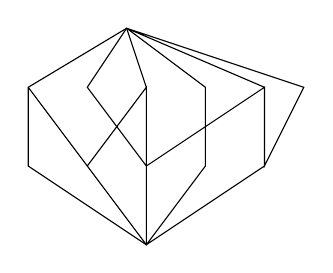
\begin{tikzpicture}[scale=.5]
\draw (11,2.5) -- (8.5,1) -- (8.5,-1) -- (11.5,-3);
\draw (8.5,1) -- (10,-1) -- (11.5,1) -- (11.5,-1) -- (10,1) -- (11,2.5) -- (13,1) -- (13,-1) -- (11.5,-3) -- (11.5,-1) -- (14.5,1) -- (14.5,-1) -- (15.5,1) -- (11,2.5) -- (14.5,1) -- (14.5,-1) -- (11.5,-3);
\draw (11,2.5) -- (11.5,1);
\draw (10,-1) -- (11.5,-3);
\vertexa at (10,-1) {};
\vertexa at (11.5,-3) {};
\vertexb at (11,2.5) {};
\vertexb at (15.5,1) {};
\vertexb at (14.5,1) {};
\vertexb at (13,1) {};
\vertexb at (11.5,1) {};
\vertexb at (10,1) {};
\vertexb at (8.5,1) {};
\vertexa at (14.5,-1) {};
\vertexa at (13,-1) {};
\vertexa at (11.5,-1) {};
\vertexa at (8.5,-1) {};
\end{tikzpicture}
\caption{The set up for Menger's $\Rightarrow$ K\"onig.}
\label{fig:konig}
\end{figure}
In fact, K\"onig's theorem is equivalent to Menger's theorem. \\
Two colorability is a rather easy property to look for. Given a graph $G$ with $n$ vertices, determining if $G$ is 2-colorable is an algorithm that runs in $n$ steps. However, the algorithm to check if a graph is even 3-colorable runs in exponential time with respect to the number of vertices, and is one of the hallmark ``NP-complete'' problems. 


\begin{comment}
\subsection{Coloring Embedded Graphs}
Historically, the problem of coloring planar graphs has been a rich field, motivated by the observation that an atlas can be colored with 4 colors. This theorem was outside the reach of mathematicians until the use of a computer program to verify a large number of edge cases. In this course, we will prove some results in the vicinity of the 4 color theorem. We start with a surprisingly useful fact about planar graphs:
\begin{lemma}
 Every simple planar graph contains a vertex of degree 5 or less.\label{lemma:lowdegree}
\end{lemma}
\begin{proof}
 We have the following inequality from before:
 \[|E|\leq 3|V|-6\]
 Assume that every vertex has degree 6 tells us $|E|\geq 3|V|$. This is a contradiction. 
\end{proof}
This allows us to run induction arguments on planar graphs where we induct on the number of vertices, and every time we remove a vertex we can choose that vertex to be of low degree. 
\begin{corollary}
 Every planar graph is 6 colorable. 
\end{corollary}
\begin{proof}
 We prove by induction on the number of vertices. \\
 Let $G$ be our graph. By Lemma \ref{lemma:lowdegree}, we can  choose to remove a vertex $v$ of degree 5. The induction hypothesis tells us that there exists a 6-coloring for $G\setminus v$. Since $v$ has degree 5, there is a color which is not used in $N(v)$. Color $v$ with that color to get a valid coloring for $G\setminus v$. 
\end{proof}

We use this to help prove the 5 color theorem. 
\begin{theorem}
 Every planar graph is 5 colorable. 
\end{theorem}
\begin{proof}
 Again, we prove by induction on removing a small degree vertex. Let $G$ be a graph, and pick a vertex $v$ of degree 5. By our induction hypothesis, we can come up with a $5$-coloring of the graph $G\setminus v$. We may assume that the neighborhood of $v$ sees all 5 colors, otherwise we would be done. As such, index $N(v)$ by colors $\{v_1, v_2, v_3, v_4, v_4\}$. Furthermore, as we are in a planar graph, we may take this labeling to proceed cyclically around $v$. We now use a trick very similar to the proof of \ref{thm:brooks}. \\
For each $i$ and $j$, let $H_{ij}$ be the $ij$ colored subgraph of $G\setminus v$. Then either $v_i$ and $v_j$ belong to the same connected component of $H_{ij}$, or not. In the case they do not, we can switch the colors $i, j$ in the connected component containing $v_i$, and now the neighborhood of $v$ only has 4 colors. \\
Suppose instead that for each $i, j$, the vertices $v_i$ and $v_j$ belong to the same connected component. This means that there is a path $P_{1,3}$ from $v_1$ to $v_3$, which is only colored with colors $1, 3$.\\
 Similarly, there must be a path $P_{2, 4}$ from $v_2$ to $v_4$ which is only colored with vertices colored $2$ and $4$. As these paths get different colors, we know that they are disjoint from each other. 
 \begin{itemize}
  \item Suppose there is not an $i,j$ colored path between $v_i$ and $v_j$ . Then $v_i$ and $v_j$ belong to separate connected components of the subgraph colored $i,j$, therefore in one component we can switch their colors, This reduces the colors in the neighborhood of $v$ to 4 colors, so we can color the graph with 5 colors. 
  \item The above must be the case, as a 13 path cannot intersect a 24 path, but the existence such paths would create a topological $K_{3,3}$ within our graph, contradicting planarity.
  \[\begin{tikzpicture}

\vertexc at (0,1) {};
\vertexa at (-2,-3) {};
\vertexd at (0,-3) {};
\vertexb at (-2,-1) {};
\vertexe at (2,-1) {};
\draw[fill=white] (0,-1) node (v1) {} circle[radius=.2];
\draw (-2,-3) -- (v1) -- (0,1);
\draw (-2,-1) -- (0,-1) -- (0,-3);
\draw (2,-1) -- (0,-1);
\node at (-2,-1.5) {$v_1$};
\node at (-0.5,0.5) {$v_2$};
\node at (1.5,-0.5) {$v_3$};
\node at (0,-3.5) {$v_4$};
\node at (-2,-3.5) {$v_5$};
\draw  plot[smooth, tension=.7] coordinates {(-2,-1) (-2,2) (0,3) (2,2) (2,-1)};
\draw  plot[smooth, tension=.7] coordinates {(0,1) (3,1) (4,-1) (3,-3) (0,-3)};

\vertexc at (3,-3) {};
\vertexd at (3,1) {};
\vertexb at (2,2) {};
\vertexe at (-2,2) {};
\node[above] at (0,3) {$P_{1,3}$};
\node[right] at (4,-1) {$P_{2,4}$};
\end{tikzpicture}\] 
 \end{itemize}
\end{proof}
There is of course the infamous 4 color theorem:
\begin{theorem}
 Every planar graph is 4 colorable. 
\end{theorem}
This theorem was historically broken by a computer, and we will not go into the proof of it here. 
\subsection{Snarks}
While the 4-coloring theorem was proven using computers, there was a different approach to proving it using a special type of graph called a \emph{snark.} Recall that an \emph{edge coloring} is an assignment of colors to the edges so that no vertex sees more than 1 of the same color edges. 
\begin{definition}
 A \emph{snark} is a 2-edge-connected graph with every vertex degree 3 and \emph{edge coloring} requiring 4 colors. 
\end{definition}
The typical example of a snark is the \emph{Peterson Graph,} which we've seen before. \\
Since the maximal degree of a vertex is three, it is obvious that we will require at least 3 colors. However, no more than 4 colors are required for the edges (the proof of this is due to Vizing's Theorem \cite{vizing1964estimate}.) \\
Not only is the Peterson graph a simple example of a snark, it is a fundamentally snarky graph:
\begin{theorem}
 Every Snark contains the Peterson graph as a minor. 
\end{theorem}
This theorem is equally as difficult to prove as the 4 color theorem. From the Snark-theorem, we can prove the 4-color theorem.
\begin{proof}[Proof of Four color theorem]
  Notice that if $G$ is a subgraph of $G'$ and $G'$ is 4 colorable, then so is $G$. We may therefore assume that our planar graph is triangulated. Furthermore, assume that the dual graph to this planar graph is again a simple graph. Notice now that $G^*$ is a cubic graph, as every face of $G$ is a triangle.\\
  We will prove by contradiction. Assume that we can show that non-existence of a 4 coloring on triangulated graph $G$. We will use this to show that $G^*$ is a cubic graph, 2-edge connected and requiring for colors, proving the $G^*$ is a snark. This means that $G^*$ contains a Peterson minor, which would imply that it contains a $K_{5}$ minor, a contradiction.  \\
   We need to show that a 3 edge-coloring of the graph $G^*$ will give me a 4 coloring of the vertices of $G$. Suppose that $E(G^*)=E_a\sqcup E_b \sqcup E_c$ is a 3-coloring of the edges.
\begin{lemma}
$G\setminus E_a$ is 2 colorable.
\end{lemma}
$G\setminus E_a$ has faces which are all 4 cycles (as they are made from 2 triangles that share a common $a$ edge). Since the faces generate the cycle space,we know that $G$ has all  even cycles. A graph with all even cycles is 2 colorable. \\
This gives us a 2-coloring to the vertices of $G\setminus E_a$, and now we would like to extend this to a coloring of $G$. Let's call the colors that we use in this coloring $\{1,2\}$. It will not extend to a valid coloring of $G$, because it may be the case that the edges in $E_a$ are monochromatic in this coloring. \\
Similarly, we know that $G\setminus E_b$ has a 2 coloring. Let's use the colors $\{3, 4\}$ in the resulting coloring. Similarly, this will not extend to a valid coloring of $G$. \\
We can combine these two 2-colorings to get a 4-coloring of $G$ using the \emph{product coloring} with colors 
\[\{12,14,23,24\}\]
Notice that this is a consistent coloring in both $G\setminus E_a$ and $G\setminus E_b$, which ends up including all of the edges. Therefore, whenever $G^*$ is 3-edge colorable, we have that $G$ is 4-colorable. 
\end{proof}
\subsection{Coloring Graphs on Surfaces}
Now I want to briefly  want to explore coloring graphs on surfaces, which is (surprisingly) completely solved. 
\begin{theorem}
 Let $\Sigma$ be an oriented surface which is not a sphere of genus $g$. Then no more than $\left \lfloor \frac{7+\sqrt{1+48g}}{2}\right \rfloor$ colors are required to color any graph on $\Sigma$. Even more surprisingly, that many colors are required in general. 
\end{theorem}
\begin{proof}
 First, we have Euler's inequality for graph, which is 
 \[|V|-|E|+|F|\geq 2-2g\]
 which tells us that 
 \[|E|\leq 3|V|+6(g-1)\]
 Let $\delta$ be the minimal degree of a vertex of $g$. Then 
 \[\delta |V|/2\leq |E|\leq 3|V|+6(g-1)\]
 which tells us that 
 \[(\delta-6)|V|\leq 12g-12\]
 because $|V|\geq \delta+1$ we have 
 \[(\delta-6)(\delta+1)\leq 12g-12\]
 which simplifies to $\delta\leq \frac{7+\sqrt{1+48g}}{2}$ giving us a minimal vertex. By the same induction argument as before, we have that every graph is at least this colorable. 
\end{proof}
\begin{elevator}[Planarity Criterion]
We provide criteria for checking whether a graph has a planar embedding. These are Kuratowski's theorem, Algebraic Planartiy criterion, and the Cycle-Cut duality criterion. 
\end{elevator}
\label{sec:planar:criterion}
In this section, we'll look at two different approaches to determining whether or not a graph admits a planar embedding. The first approach looks for topological minors of $G$ which are ``obstructions'' to finding a planar drawing. This method basically tries to construct a drawing of the graph according to an algorithm, and classifies the types of topological minors that prevent the algorithm from running.\\
The second approach asks what kind of algebraic data one can get about a graph by looking at the faces of the planar embedding, and whether the existence of such data guarentees a planar embedding. \\
Finally, we'll take a look again at dual graphs, and show that being planar is, in the appropriate language, equivalent to having a dual graph. 
\subsection{Kuratowski's Theorem}

 $K_{3,3}$ and $K_5$ form the essential obstruction to a graph being planar. 
\begin{theorem}[\cite{kuratowski1930probleme}]\label{thm:kuratowski}
 The following are equivalent:
 \begin{itemize}
  \item $G$ is planar
  \item $G$ contains $K_{3,3}$ or $K_{5,5}$ as a topological minor.
  \item $G$ contains $K_{3,3}$ or $K_{5,5}$ as a minor.
 \end{itemize}
\end{theorem}
We will prove a number of proposition about $K_5$ and $K_{3,3}$ first.
\begin{prop}
 If $\Delta(G)$, the maximal degree of $G$ is at most 3, then the following are equivalent:
 \begin{itemize}
  \item $G$ is a topological minor of $H$.
  \item $G$ is a minor of $H$. 
 \end{itemize}
\end{prop}
\begin{proof}
See Exercise \ref{exer:3minors}
\end{proof}

\begin{prop}
	The following are equivalent:
	\begin{itemize}
	 \item $G$ contains $K_5$ or $K_{3,3}$ as a topological minor.
	 \item $G$ contains $K_5$ or $K_{3,3}$ as a minor. 
	\end{itemize}
\end{prop}
\begin{proof}
 By Exercise \ref{exer:3minors}, if $G$ contains $K_{3,3}$ as a minor, it contains it as a topological minor. \\
 So, we only need to show that if $G$ contains $K_5$ as a minor then it contains $K_5$ or $K_{3,3}$ as a topological minor. Let $H$ be a minimal subgraph of $G$ which contains $K_5$ as a minor. Each vertex in the $K_5$ corresponds to a ``blob'' in the subgraph $H$. Now, it is either the case that in each blob there is a vertex of degree 4, or there are 2 vertices of degree 3. 
 \begin{itemize}
 \item If every blob contains a vertex of degree 4, then we have that $H$ is a subdivision of $K_5$. 
 \item If a blob contains a vertex of degree 3, then $H$ contains $K_{3,3}$ as a minor. See Figure \ref{fig:k33k5} for a diagram of that minor. 
 \end{itemize}
\end{proof}
\begin{figure}
\centering
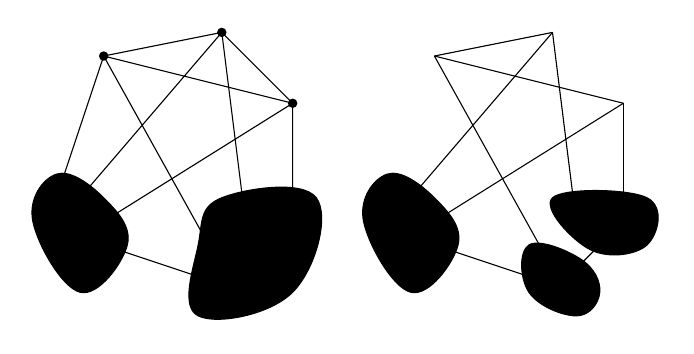
\begin{tikzpicture}[scale=.6]

\draw  [fill=\shadinga]  plot[smooth cycle, tension=.7] coordinates {(7.5,-1.5) (8.6,-1.8) (9,-2.5) (8.5,-3) (7.5,-2.5)};
\draw [fill=\shadinga] plot[smooth cycle, tension=.7] coordinates {(4.5,0) (4,-1) (5,-2.5) (6,-1.5) (5.5,-0.5)};
\draw [fill=\shadinga]  plot[smooth cycle, tension=.7] coordinates { (8.8,-1.6) (10,-1.5) (10,-0.5) (8,-0.5)};

\draw [fill=\shadinga] plot[smooth cycle, tension=.7] coordinates {(-2.5,0) (-3,-1) (-2,-2.5) (-1,-1.5) (-1.5,-0.5)};
\draw [fill=\shadinga]  plot[smooth cycle, tension=.7] coordinates {(0.5,-1.5) (0.5,-3) (2.5,-2.5) (3,-0.5) (1,-0.5)};

\draw (-2,-1.5);
\draw (-2,-1.5) -- (-2.5,-0.5) -- (-1.5,2.5) -- (1,3) -- (2.5,1.5) -- (2.5,-1) -- (2,-1.5) -- (1.5,-1) -- (1,3) -- (-2,-0.5) -- (-2,-1.5) -- (-1.5,-1) -- (2.5,1.5) -- (-1.5,2.5) -- (1,-2) -- (1.5,-2) -- (1.5,-2.5) -- (-1.5,-1.5);
\draw (1.5,-2) -- (2,-1.5);
\draw (-1.5,-1.5) -- (-2,-1.5);
\draw (8.5,-2);
\draw (8.5,-2) --  (9,-1.5) ;
\draw (9.5,-1) -- (9.5,1.5);
\draw (8,3) -- (8.5,-1);
\draw (8.5,-2.5) -- (5.5,-1.5);
\draw (8,-2) -- (5.5,2.5);
\draw (8,-2);
\draw (8,-2) -- (8.5,-2) -- (8.5,-2.5);
\draw (9.5,1.5) -- (5.5,-1) -- (5,-1.5) -- (5,-0.5) -- (8,3);
\draw (5.5,2.5) -- (8,3);
\draw (5.5,2.5) -- (9.5,1.5);
\draw (4.5,-0.5) -- (5,-1.5) -- (5.5,-1.5);
\draw (8.5,-1) -- (9,-1.5) -- (9.5,-1);
\fill (1.5,-2) circle[radius=.1];
\fill (1.5,-1) circle[radius=.1];
\fill (2,-1.5) circle[radius=.1];
\fill (2.5,-1) circle[radius=.1];
\fill (2.5,1.5) circle[radius=.1];
\fill (1,3) circle[radius=.1];
\fill (-1.5,2.5) circle[radius=.1];
\fill (-2,-0.5) circle[radius=.1];
\fill (-2,-1.5) circle[radius=.1];
\fill (-1.5,-1.5) circle[radius=.1];
\fill (-1.5,-1) circle[radius=.1];
\fill (-2.5,-0.5) circle[radius=.1];
\fill (1.5,-2.5) circle[radius=.1];
\fill (1,-2) circle[radius=.1];
\vertexa  (8.5,-2) {};
\vertexb  (8.5,-1) {};
\vertexb  (9,-1.5) {};
\vertexb  (9.5,-1) {};
\vertexa  (9.5,1.5) {};
\vertexa  (8,3) {};
\vertexb at (5.5,2.5) {};
\vertexb  (5,-0.5) {};
\vertexb  (5,-1.5) {};
\vertexb  (5.5,-1.5) {};
\vertexb  (5.5,-1) {};
\vertexb  (4.5,-0.5) {};
\vertexa  (8.5,-2.5) {};
\vertexa  (8,-2) {};
\end{tikzpicture}
\caption{If the contraction merges together 2 vertices of degree 3 in the $K_5$, then there exists a $K_{3,3}$ minor. }
\label{fig:k33k5}
\end{figure}

We start with a proof of Kuratowski's theorem for 3-connected graphs using the contraction lemma that we have. 
\begin{lemma}
 Every non-planar 3-connected graph contains $K_{3,3}$ or $K_5$ as a minor. 
\end{lemma}

\begin{proof}
 We induct on the number of edges in the graph.

\begin{tabular}[t]{p{.5 \textwidth}r}
By Lemma \ref{lemma:3connect}, we can find an edge $xy$ so that $G/xy$ is still 3-connected. & 
 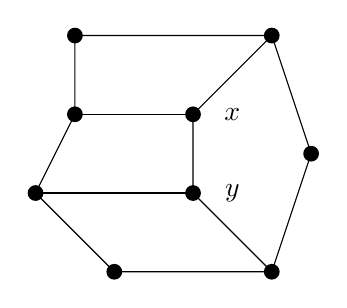
\begin{tikzpicture}[baseline=(current bounding box.north)]
\fill (-2,-0.5) circle[radius=.1];
\fill (-3.5,-0.5) circle[radius=.1];
\fill (-0.5,-1) circle[radius=.1];
\fill (-2,-1.5) circle[radius=.1];
\fill (-1,0.5) circle[radius=.1];
\fill (-3.5,0.5) circle[radius=.1];
\fill (-1,-2.5) circle[radius=.1];
\fill (-3,-2.5) circle[radius=.1];
\fill (-4,-1.5) circle[radius=.1];
\draw (-1,0.5) -- (-3.5,0.5) -- (-3.5,-0.5) -- (-4,-1.5) -- (-3,-2.5) -- (-1,-2.5) -- (-0.5,-1) -- (-1,0.5) -- (-2,-0.5) -- (-2,-1.5) -- (-1,-2.5);
\draw (-3.5,-0.5) -- (-2,-0.5);
\draw (-2,-1.5) -- (-4,-1.5);
\node at (-1.5,-0.5) {$x$};
\node at (-1.5,-1.5) {$y$};
\end{tikzpicture} \\
By induction hypothesis, $G/xy$ is 3 connected and has a planar drawing. Let's look at that planar drawing. Let $C$ be the set of vertices which belong to a face that $v_{xy}$ does. This set is necessarily a walk (as it is the boundary of a collection of faces) but since $G/xy$ is 3 connected, we know that it is in fact a cycle.     &
 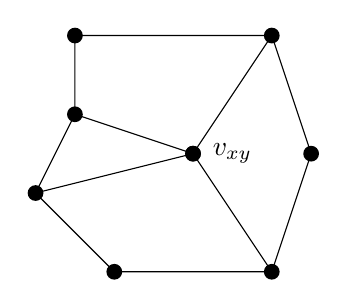
\begin{tikzpicture}[baseline=(current bounding box.north)]
\fill (3,-1) circle[radius=.1];
\fill (1.5,-0.5) circle[radius=.1];
\fill (4.5,-1) circle[radius=.1];
\fill (3,-1) circle[radius=.1];
\fill (4,0.5) circle[radius=.1];
\fill (1.5,0.5) circle[radius=.1];
\fill (4,-2.5) circle[radius=.1];
\fill (2,-2.5) circle[radius=.1];
\fill (1,-1.5) circle[radius=.1];
\draw (4,0.5) -- (1.5,0.5) -- (1.5,-0.5) -- (1,-1.5) -- (2,-2.5) -- (4,-2.5) -- (4.5,-1) -- (4,0.5) -- (3,-1) -- (3,-1) -- (4,-2.5);
\draw (1.5,-0.5) -- (3,-1);
\draw (3,-1) -- (1,-1.5);
\node at (3.5,-1) {$v_{xy}$};
\end{tikzpicture}\\
The collection $C$ is the boundary of a face in the planar drawing of $G/xy \setminus v_{xy}$. We can now try adding in the the edge $xy$ and other edges of $G$. In this simplified case, we can to a case by case analysis to the obstruction of a planar embedding. Each case results in the creation of a $K_{3,3}$ or $K_5$ minor. (To check the cases, try adding in edges in clockwise order coming from $C$.) &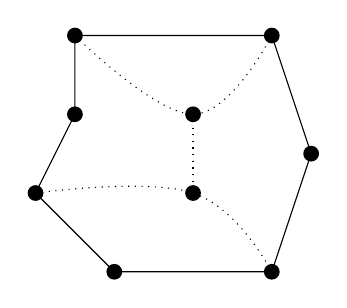
\begin{tikzpicture}[baseline=(current bounding box.north)]
\fill (8,-0.5) circle[radius=.1];
\fill (8,-1.5) circle[radius=.1];
\fill (6.5,-0.5) circle[radius=.1];
\fill (9.5,-1) circle[radius=.1];
\fill (9,0.5) circle[radius=.1];
\fill (6.5,0.5) circle[radius=.1];
\fill (9,-2.5) circle[radius=.1];
\fill (7,-2.5) circle[radius=.1];
\fill (6,-1.5) circle[radius=.1];
\draw (9,0.5) -- (6.5,0.5) -- (6.5,-0.5) -- (6,-1.5) -- (7,-2.5) -- (9,-2.5) -- (9.5,-1) -- (9,0.5);

\draw[dotted]  plot[smooth, tension=.7] coordinates {(6,-1.5) (8,-1.5) (9,-2.5)};
\draw[dotted]  plot[smooth, tension=.7] coordinates {(6.5,0.5) (8,-0.5) (9,0.5)};
\draw[dotted] (8,-0.5) -- (8,-1.5);
\end{tikzpicture}
\end{tabular}\\
\begin{figure}
\centering
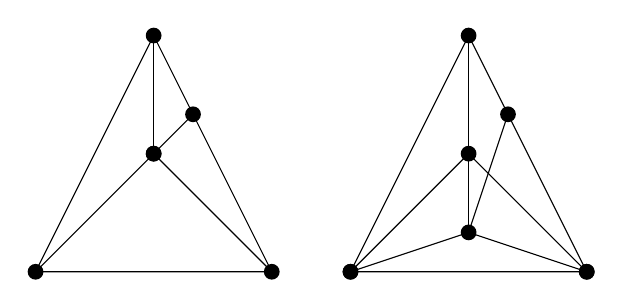
\begin{tikzpicture}

\fill(-7.5,0.5) circle[radius=.1];
\fill(-7.5,-1) circle[radius=.1];
\fill(-7.5,-1) circle[radius=.1];
\fill(-6,-2.5) circle[radius=.1];
\fill(-9,-2.5) circle[radius=.1];
\fill(-7,-0.5) circle[radius=.1];
\draw (-7.5,0.5) -- (-9,-2.5) -- (-6,-2.5) -- (-7.5,0.5);
\draw (-9,-2.5) -- (-7.5,-1) -- (-6,-2.5);
\draw (-7.5,-1) -- (-7.5,-1);
\draw (-7.5,-1) -- (-7.5,0.5);
\draw (-7.5,-1) -- (-7,-0.5);
\fill(-3.5,0.5) circle[radius=.1];
\fill(-2,-2.5) circle[radius=.1];
\fill(-3.5,-2) circle[radius=.1];
\fill(-3.5,-1) circle[radius=.1];
\fill(-2,-2.5) circle[radius=.1];
\fill(-5,-2.5) circle[radius=.1];
\fill(-5,-2.5) circle[radius=.1];
\fill(-3,-0.5) circle[radius=.1];
\draw (-3.5,0.5) -- (-5,-2.5) -- (-2,-2.5) -- (-3.5,0.5);
\draw (-5,-2.5) -- (-3.5,-1) -- (-2,-2.5);
\draw (-3.5,-2) -- (-3.5,-1);
\draw (-5,-2.5) -- (-3.5,-2) -- (-2,-2.5);
\draw (-3.5,-1) -- (-3.5,0.5);
\draw (-3.5,-2) -- (-3,-0.5);
\end{tikzpicture}\caption{An obstruction to coloring adding in the edge that gives us the topological $K_5$. }
\end{figure}
\begin{figure}
\centering
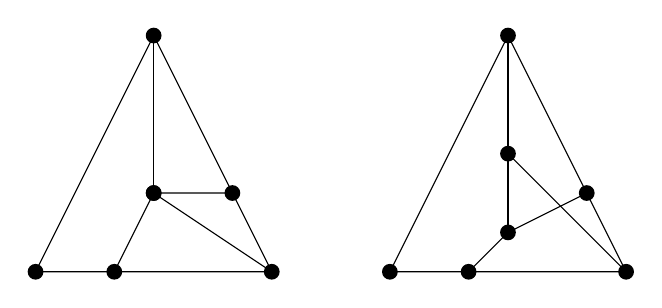
\begin{tikzpicture}
\fill(-3.5,0.5) circle[radius=.1];
\fill(-2.5,-1.5) circle[radius=.1];
\fill(-3.5,-1.5) circle[radius=.1];
\fill(-3.5,-1.5) circle[radius=.1];
\fill(-2,-2.5) circle[radius=.1];
\fill(-5,-2.5) circle[radius=.1];
\fill(-4,-2.5) circle[radius=.1];
\draw (-3.5,0.5) -- (-5,-2.5) -- (-2,-2.5) -- (-3.5,0.5);
\draw   (-3.5,-1.5) -- (-2,-2.5);
\draw (-3.5,-1.5) -- (-3.5,-1.5);
\draw (-4,-2.5) -- (-3.5,-1.5) -- (-2.5,-1.5);
\draw (-3.5,-1.5) -- (-3.5,0.5);
\fill(1,0.5) circle[radius=.1];
\fill(2,-1.5) circle[radius=.1];
\fill(1,-2) circle[radius=.1];
\fill(1,-1) circle[radius=.1];
\fill(2.5,-2.5) circle[radius=.1];
\fill(-0.5,-2.5) circle[radius=.1];
\fill(0.5,-2.5) circle[radius=.1];
\draw (1,0.5) -- (-0.5,-2.5) -- (2.5,-2.5) -- (1,0.5);
\draw   (1,-1) -- (2.5,-2.5);
\draw (1,-2) -- (1,-1);
\draw (0.5,-2.5) -- (1,-2) -- (2,-1.5);
\draw (1,-1) -- (1,0.5);

\end{tikzpicture}
\caption{An obstruction to adding in the edge that gives us a topological $K_{3,3}$. }
\end{figure}
\end{proof}

\begin{corollary}
 Suppose $G$ is 3-connected and planar. Then there exists a drawing of $G$ which has all convex faces. 
\end{corollary}
\begin{proof}
 We induct on the number of edges as before. The base case is $K_4$, and this graph is clearly connected. \\
 Pick $xy$, an edge of $G$ so that $G/xy$ is still 3-connected. By the induction hypothesis, there exists an embedding of $G/xy$ so that every face is convex. We can treat the vertex $v_{xy}$ as the vertex $x$. The addition of a vertex and edges to the center of any convex face can be done in such a way that every additional edge creates a convex face. 
\end{proof}
This means that in particular every single planar graph which is 3 connected can be drawn with straight edges. In fact, every planar graph can be drawn with straight edges. \\
We now have enough machinery to prove Kuratowski's theorem. 
\begin{proof}[Proof of Theorem \ref{thm:kuratowski}]
 We may assume that $G$ is 2 connected. Let $x,y$ be a cutset of $G$ so that 
 \[G=G_1\cup G_2 \;\;\;\;\;G_1\cap G_2=\{x,y\}\]
 Then if $G$ does not contain a topological $K_{3,3}$ or a $K_5$, neither does $G_1\cup xy$ or $G_2\cup xy$. This is because there is a path from $x$ to $y$ in both $G_1$ and $G_2$. 
 Therefore by induction there exits a planar drawing of both $G_1+xy$ and $G_2+xy$. We can assume that these drawings both have $xy$ as an exterior edge-- gluing along this edge yields a planar drawing of $G$.
\end{proof}
The search for a topological $K_5$ or $K_{3,3}$ seems like a difficult thing to do in a graph. There is an algebraic criterion for planarity of a graph as well, which is easier to check.


\subsection{Algebraic Planarity}

Recall we had previously defined a \emph{chain complex} associated to a planar graph (Definition \ref{def:graphcomplex}.)
\[ \begin{tikzcd} 
\mathcal F \arrow{r}{\partial_F}& \mathcal E \arrow{r}{\partial_E}& \mathcal V 
\end{tikzcd}\]

 This chain complex gives us additional structure on the cycle space. In Claim \ref{claim:dsquarezerograph}, we showed that $\im \partial_F\subset \ker \partial_E$. This means that some of the cycles of $G$ are described by the faces. In fact, in a planar graph, every cycle is described by the faces, which \emph{nearly} a basis. 
\begin{definition}
 A subspace $\mathcal U\subset \mathcal E$ is called \emph{simple} if there exists a basis $\mathcal B$ for $\mathcal U$ with the following property: Let $E(U)$ be the set of all edges which appear in elements of $E$. Let $b_1, \ldots, b_k\in \mathcal B$ be our basis. Then there exists another element $b_0$ so every element $e\in E(U)$ appears in exactly two of the $b_i$. 
\end{definition}

\begin{theorem}
 A graph is planar if and only if there is a simple basis for the cycle space. 
\end{theorem}
\begin{proof}
 In the case of planarity, choose a basis given by the faces of some planar embedding of $G$. Let $f_0, f_1, \ldots, f_k$ be the faces of $G$, where $f_0$ is the outside face. Let $\mathcal B = \{\partial_F(f_i)\;|\; i\geq 1\}$. This forms a basis, as every cycle can be written as the sum of the faces which are on the interior of that cycle. Similarly, every edge only belongs to 2 faces, so the resulting basis we have is simple.  \\ 
 \begin{figure}
 \centering
 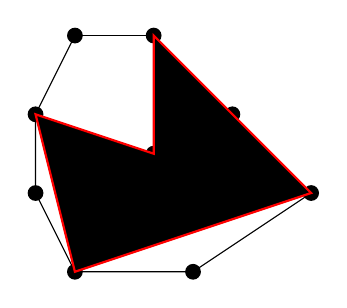
\begin{tikzpicture}
\fill[\shadinga] (-3,-4.5) -- (-3,-6) -- (-4.5,-5.5) -- (-4,-7.5) -- (-1,-6.5) -- (-2,-5.5) -- cycle;
\fill (-2,-5.5)  circle[radius=.1];
(-4,-7.5) -- (-1,-6.5) -- (-2,-5.5) -- cycle;
\fill (-4,-4.5) circle[radius=.1];
\fill (-4.5,-5.5) circle[radius=.1];
\fill (-3,-6) circle[radius=.1];
\fill (-1,-6.5) circle[radius=.1];
\fill (-3,-4.5) circle[radius=.1];
\fill (-2.5,-7.5) circle[radius=.1];
\fill (-4,-7.5) circle[radius=.1];
\fill (-4.5,-6.5) circle[radius=.1];
\draw (-4,-4.5) -- (-4.5,-5.5) -- (-4.5,-6.5) -- (-4,-7.5) -- (-2.5,-7.5) -- (-1,-6.5) -- (-2,-5.5)  -- (-3,-6) -- (-1,-6.5) -- (-4,-7.5) -- (-4.5,-5.5) -- (-3,-6) -- (-3,-4.5) -- (-2,-5.5);
\draw (-4,-4.5) -- (-3,-4.5);
\draw[red, thick] (-3,-4.5) -- (-3,-6) -- (-4.5,-5.5) -- (-4,-7.5) -- (-1,-6.5) -- (-2,-5.5) -- cycle;
\end{tikzpicture}
\caption{Every cycle is written as the sum of the boundary cycles of the interior faces.}
\end{figure}
We now are ready to show that having a simple basis implies planarity. Since planarity is equivalent to containing a topological $K_{3,3}$ or $K_5$ minor (Theorem \ref{thm:kuratowski}.) Therefore, we can prove the contrapositive statement: that containing a topological $K_{3,3}$ and $K_5$ implies you are non-simple. \\
 First notice if $G$ has a simple basis, and $H$ is a subdivision of $G$, then $G$ has a simple basis if and only if $H$ has a simple basis. This is because the cycle spaces of topological subdivisions are isomorphic, and subdivision preserves the simple basis property. \\
 Similarly, one can check that $G\subset H$, then $G$ admits a simple basis whenever  $H$ has a simple basis. This is in Exercise \ref{exer:simplebasis}. Now we know that whenever $G$ is a topological minor of $H$, a simple basis for $H$ gives us a simple basis for $G$.  \\
 Let's do $K_5$ first. By Exercise \ref{exer:b0kn} we have that $\dim(\mathcal C(K_5)=6$. Therefore any basis has 6 elements in it. Being simple means that we have a set $\{c_0, \ldots, c_6\}$ which contains edges 0 or 2 times. Since each cycle has 3 edges, the collection $\{c_0, \ldots, c_6\}$ has at least $7\cdot 3 = 21$ edges. However there are only 10 edges in $K_5$, a contradiction.\\
 Similarly, we've computed that for $K_{3,3}$, we know that the cycle space has dimension 4. Given some basis of 4 elements, we have an additional element $C$ so that the collection of basis elements and $C$ represents every edge exactly two or 0 times. The collection of 5 cycles contains 20 edges, because each cycle has length at least 4. But there are 9 edges total, so again creates a counting problem. 
\end{proof}

Ok, so we've finished the algebraic criteria for planarity. One unfortunate thing about this proof is that we have to use Kuratowski's theorem to finish it-- ideally we would have a proof of this theorem that avoids the use of Kuratowski's theorem, and this proof would generalize to graphs embedding in other surfaces by looking at the faces that come from those embeddings.\\
A nice interpretation of the algebraic planarity criterion comes from studying dual graphs of planar graphs (Definition \ref{def:dualgraph})
\begin{definition}
Let $G$ be a connected graph. Let $V=V_1\sqcup V_2$. The \emph{cut set} between $V_1$ and $V_2$ is the subset of all edges between vertices of $V_1$ and $V_2$. We denote such a cutset as $E(V_1, V_2)$. We say that a cut set is \emph{minimal} if it belongs to no other cutsets. 
\end{definition}
\examplefigure{Here is an example of a graph $G$ with a partition of it's vertices into $V_1$ and $V_2$. The graph $G$ decomposes into the induced subgraph on the vertex subsets, plus a collection of edges that go in between those two subgraphs. }{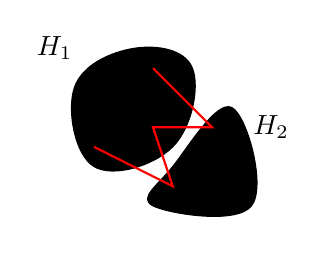
\begin{tikzpicture}[scale=.5]

\draw[fill=\shadinga]  plot[smooth cycle, tension=.7] coordinates {(7,-1) (7.5,-3) (9.5,-2.5) (10,-0.5) (8.5,0)};
\draw[fill=\shadinga]  plot[smooth cycle, tension=.7] coordinates {(11,-1.5) (9.5,-3) (9,-4) (11.5,-4)};
\fill (9,-2) circle[radius=.1];
\fill (11,-3.5) circle[radius=.1];
\fill (10.5,-2) circle[radius=.1];
\fill (9.5,-3.5) circle[radius=.1];
\fill (9,-0.5) circle[radius=.1];
\fill (7.5,-1.5) circle[radius=.1];
\fill (7.5,-2.5) circle[radius=.1];
\draw (7.5,-2.5) -- (7.5,-1.5) -- (9,-0.5) -- (9,-2) -- (7.5,-2.5) -- (9,-0.5);
\draw (10.5,-2) -- (9.5,-3.5) -- (11,-3.5) -- (10.5,-2);
\draw[red, thick] (7.5,-2.5) -- (9.5,-3.5) -- (9,-2) -- (10.5,-2) -- (9,-0.5);
\node at (6.5,0) {$H_1$};
\node at (12,-2) {$H_2$};
\end{tikzpicture}}

Cut sets behave in a lot of ways similar to cycles. Define the \emph{  cut space} $\mathcal C^*\subset \mathcal E$ as the set of all cuts. In many ways it is better behaved than the cycle space, as it is a space of its own right (we don't need to take span). To prove this observe that 
\begin{claim}
 Cuts of the from $E(v, G\setminus v)$ span the cut space.  The cut space has a simple basis of the form $E(v, G\setminus v).$
\end{claim}
\begin{proof}
 Given any cut $E(H_1, H_2)$, let $v$ be a vertex of $H_1$. Observe that $ E(H_1, H_2)=E(H_1\setminus v, H_2\cup v)+E(v, G\setminus v)$. This means that 
 \[E(H_1, H_2)=\sum_{v\in H_1} H(v, G\setminus v). \]
 This shows that the vertices $v$ span the cutset, so certainly some subset of them form a basis. Since each edge belongs to at most 2 sets of the form $E(v, G\setminus v)$, we get that the resulting basis is simple. 
\end{proof}
The cut space serves as a natural dual to the cycle space. The \emph{standard inner product} on $\mathcal E$ is the dot product of edge sets when written in coordinates coming from the basis of edges.  With this inner product, 
\[b_1\cdot b_2=\text{Number of edges that $b_1$ and $b_2$ share in common, $\mod 2$}\]
\begin{claim}
 With the standard inner product on $\mathcal E$, we have that $(C)^\bot=C^*$.
\end{claim}
\begin{proof}
 To show that $\mathcal C\subset \mathcal( C^*)^\bot$, it suffices to show that every cycle shares an even number of edges with each cut. If you think of a cut describing the edges that go between $H_1$ and $H_2$, it is clear that a cycle must cross those edges an even number of times. So the inclusion is proved. \\
 Now to show that $\mathcal C^*=\mathcal C^\bot$, we need to show that $E\not \in \mathcal C$ implies that $E\cdot F\neq 0$ for some cut set $F$. Now, if $E$ is not a sum of cycles, then there is a vertex which shares an odd number of edges with $E$. This is because every cycle has even degree on every vertex. Now this vertex has a cut set $F$ which has $E\dot F=1$. This shows the other inclusion. 
\end{proof}
Unlike in the case of the cycle space, the cut set comes with a simple generating set. 


\begin{definition}
 We say that two multigraphs $G$ and $G^*$ are \emph{abstract dual} if there is a bijection of the edges so that $\mathcal C_G=\mathcal C_{G^*}^*$. 
\end{definition}
\begin{claim}
 $G$ and $G^*$ planar dual implies that $G$ and $G^*$ are abstract dual. 
\end{claim}
\examplefigure{In this example, we've drawn two dual polytopes: the octahedron in black, and the cube in red. The collection of faces shaded in gray represent a cycle in the octahedron, giving us the corresponding cut set (demarcated with dashes) in the cube.}{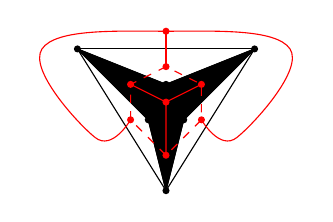
\begin{tikzpicture}[scale=.45]
\draw[fill=\shadinga] (-6.5,-5) -- (-4.5,-7) -- (-4,-9) -- (-3.5,-7) -- (-1.5,-5) -- (-4,-6) -- (-6.5,-5);
\fill (-4,-6) circle[radius=.1];
\fill (-3.5,-7) circle[radius=.1];
\fill (-1.5,-5) circle[radius=.1];
\fill (-6.5,-5) circle[radius=.1];
\fill (-4,-9) circle[radius=.1];
\fill (-4.5,-7) circle[radius=.1];
\draw (-6.5,-5) -- (-4.5,-7) -- (-4,-6) -- (-3.5,-7) -- (-1.5,-5) -- (-4,-6) -- (-6.5,-5);
\draw (-3.5,-7) -- (-4.5,-7) -- (-4,-9) -- (-3.5,-7);
\draw (-1.5,-5) -- (-4,-9);
\draw (-6.5,-5) -- (-4,-9);
\draw (-6.5,-5) -- (-1.5,-5);



%cube

\fill[red] (-4,-5.5) circle[radius=.1];
\fill[red] (-4,-4.5) circle[radius=.1];
\fill[red] (-4,-8) circle[radius=.1];
\fill[red] (-3,-7) circle[radius=.1];
\fill[red] (-5,-7) circle[radius=.1];
\fill[red] (-3,-6) circle[radius=.1];
\fill[red] (-5,-6) circle[radius=.1];
\fill[red] (-4,-6.5) circle[radius=.1];
\draw[dashed, red] (-4,-5.5) -- (-5,-6) -- (-5,-7) -- (-4,-8) -- (-3,-7) -- (-3,-6) -- (-4,-5.5);
\draw[red] (-5,-6) -- (-4,-6.5) -- (-4,-8);
\draw[red] (-3,-6) -- (-4,-6.5);
\draw[red]  plot[smooth, tension=.7] coordinates {(-5,-7) (-6,-7.5) (-7.5,-5) (-4,-4.5) (-0.5,-5) (-2,-7.5) (-3,-7)};
\draw[red] (-4,-5.5) -- (-4,-4.5);
\end{tikzpicture}}
\begin{proof}
 Let $F\subset E_G$ be a minimal edge cut that separates $G$. This creates 2 components. The intersection of all the faces contained in one region and contained in the other region should have the property that each face only contains 2 edges from the minimal cut set-- as only 2 edges are required separate the cycle which is each face. This means that we have a collection of faces which all have degree 2 in the dual. This gives us a collection of cycles. Of course, it can't be a collection of cycles, as this would cause various separate regions by the Jordan curve theorem. 
\end{proof}
The other direction is clear.  This means that whenever $G$ and $G^*$ planar dual imply that $G$ and $G^*$ are abstract dual. Furthermore, since planar duality is actually a duality, we get for free that $(G^*)^*=G$. For this reason, we haven't been distinguishing between abstract duality and planar duality in notation. This is in fact and equivalence, as abstract duality is equivalent to planarity. 
\begin{theorem}[Whitney]
 A graph is planar if and only if it has an abstract dual.
\end{theorem}
\begin{proof}
 The forward direction we just proved-- the dual multigraph is a candidate dual. For the other direction, notice that the cut space of $G^*$ has a simple basis, therefore the cycle space of $G$ has a simple basis, therefore $G$ is planar. 
\end{proof}
In fact, this kind of duality shows up in a lot of different places in combinatorics. At its heart, planar duality, abstract duality and cycles and cut-sets are the first shadows of a \project larger class of combinatorial objects called \emph{matroids.} \label{proj:matroids.} These generalizations of graphs capture the idea of relations by looking at ``linearly independent sets'' within some collection that one studies. \\
Similarly, the duality has a topological meaning, in the form of \emph{Poincar\'e duality.} On compact oriented $n$- manifolds, the space of $k$ cycles looks very \project much like the space of $n-k$ cycles, and there is a pairing between them in very much the same way that there is a pairing between cut sets and cycles. While we won't have time to go into this general phenomenon in this course, it would be an interesting thing to look at. 

\end{comment}